\documentclass{article}
\usepackage{titlesec}
\usepackage{titling}
\usepackage{float}
\usepackage{listings}
\usepackage{xcolor}
\usepackage{graphicx}
\usepackage{hyperref}
\usepackage{xepersian}

\renewcommand{\labelitemi}{$\circ$}
\renewcommand{\labelitemii}{$\circ$}
\renewcommand{\labelitemiii}{$\circ$}
\renewcommand{\labelitemiv}{$\circ$}



\setlatintextfont[Scale=0.85]{Noto Sans}

\settextfont{B Nazanin}
\title{
\includegraphics[width=1in,height=1in]{logo.png}
	\\[1cm]
	چالش سوم: \lr{M5 Forecasting - Accuracy} }
\author{فراهم‌آورنده: سینا حیدری}
\date{زمستان ۹۸}

\definecolor{codegreen}{rgb}{0,0.6,0}
\definecolor{codegray}{rgb}{0.5,0.5,0.5}
\definecolor{codepurple}{rgb}{0.58,0,0.82}
\definecolor{backcolour}{rgb}{0.95,0.95,0.92}

\lstdefinestyle{mystyle}{
	backgroundcolor=\color{backcolour},   
	commentstyle=\color{codegreen},
	keywordstyle=\color{magenta},
	numberstyle=\tiny\color{codegray},
	stringstyle=\color{codepurple},
	basicstyle=\ttfamily\footnotesize,
	breakatwhitespace=false,         
	breaklines=true,                 
	captionpos=b,                    
	keepspaces=true,                 
	numbers=left,                    
	numbersep=5pt,                  
	showspaces=false,                
	showstringspaces=false,
	showtabs=false,                  
	tabsize=2
}

\lstset{style=mystyle}

\titlespacing*{\section}{0pt}{50pt}{40pt}
\begin{document}
	\maketitle
	\newpage
	\ \\
	برای مشاهده‌ی جزئیات این چالش در کگل به لینک زیر مراجعه کنید.\\
\begin{flushleft}
	\href{https://www.kaggle.com/c/m5-forecasting-accuracy}{\lr{https://www.kaggle.com/c/m5-forecasting-accuracy}}
\end{flushleft}
\section{در مورد این چالش}
نکته: این رقابت یکی از سه رقابتی است که چالش \lr{M5 forcasting} را تشکیل می‌دهد. آیا می‌توانید با دقت بالا، تعداد واحدهایی از هر محصول، که توسط وال‌مارت در آمریکا به‌فروش خواهد رفت را پیش‌بینی کنید؟
\ \\
یک فروشگاه، چه تعداد ابزار چادرزنی را، در هر ماه از سال خواهد فروخت؟ برای کسانی که دانش پیشین ندارند، محاسبه‌ی فروش‌ها در این سطح به‌اندازه‌ی پیش‌بینی آب‌وهوا سخت جلوه می‌کند. هر دو نوع پیش‌بینی\footnote{\lr{forcasting}}، وابسته به دانش و داده‌های مبتنی بر تاریخ است. یک پیش‌بینی اشتباه آب‌وهوا شاید باعث شود چترتان را در یک روز آفتابی بدون استفاده با خود حمل کنید؛ اما یک پیش‌بینی اشتباه در کسب‌وکار ممکن است موجب از دست رفتن فرصت‌های واقعی شود. در این رقابت، علاوه بر روش‌های سنتی پیش‌بینی، از \textbf{یادگیری ماشین} هم برای بالا بردن دقت پیش‌بینی‌ها بهره می‌بریم.
\ \\
مرکز پیش‌بینی ماکریداکیس (\lr{MOFC}) در دانشگاه نیکوزیا تحقیقات پیشرفته‌یی را در زمینه‌ی پیش‌بینی هدایت کرده و آموزش پیش‌بینی‌ کسب‌وکار را فراهم می‌آورد. این مرکز به‌شرکت‌ها کمک می‌کند تا به پیشبینی‌های دقیق دست یافته؛ درجات عدم‌قطعیت را تقریب زده، از اشتباهات هزینه‌بر دوری کرده، و بهترین روش‌های پیش‌بینی را در کسب‌وکارشان اعمال کنند. \lr{MOFC} به‌دلیل رقابت‌های \lr{Makridakis}-که اولین رقابت‌اش در سال ۱۹۸۰ برگذار شد-در دنیا به خوبی شناخته شده است.
\ \\
در این رقابت از داده‌ی سلسله‌مراتبی فروش‌های \textbf{وال‌مارت}-که از بزرگ‌ترین شرکت‌های دنیا است-برای پیش‌بینی روزانه‌ی فروش‌ها، در ۲۸ روز آینده استفاده کرده و برای این پیش‌بینی‌ها عدم‌قطعیت را تقریب بزنیم. مجموعه‌داده، فروشگاه‌های داخل سه ایالت آمریکا (کالیفرنیا، تگزاس و ویسکانسین) را در بر گرفته و شامل درجه‌ی آیتم، دپارتمان، دسته‌بندی محصول و جزئیات فروشگاه می‌شود. علاوه بر این، شامل مقادیر توضیحی، همچون؛ قیمت، تبلیغات، روز هفته و رخدادهای خاص می‌شود. از تمام این‌ها می‌توان استفاده کرد تا دقت پیش‌بینی را افزایش داد. 
\ \\
اگر موفق باشیم، کارمان در مسیر پیشرفت تئوری و عملی پیش‌بینی جلو خواهد رفت. روش‌های استفاده شده را می‌توان برای راه‌اندازی مناسب انبارها یا درجه‌های سرویس‌دهی به‌کار برد. \lr{MOFC} از طریق حمایت و آموزش به توزیع ابزار‌ها و دانش کمک می‌کند تا بقیه هم بتوانند به‌دقت بالاتر و درجه‌بندی بهتر پیش‌بینی دست یافته، ضایعات را کاهش دهند و آمادگی پذیرفتن ریسک‌های عدم‌قطعیت را داشته باشند.
\section{در مورد این گزارش}
در این گزارش، ساختار داده را به‌طور خلاصه توصیف می‌کنیم. سپس، داده را با استفاده از دو کتابخانه‌ی \lr{Matplotlib} و \lr{Plotly} مصورسازی می‌کنیم. در نهایت، نشان خواهیم چه رویکردهایی به این مسئله از طریق الگوریتم‌‌های پیش‌بینی وجود دارد. 
\section{بررسی اکتشافی داده}
داده‌ی ما شامل پنج فایل می‌شود:
\begin{flushleft}
\begin{latin}
\begin{itemize}
\item
\textbf{calendar.csv} - Contains the dates on which products are sold. The dates are in a yyyy/dd/mm format.
\item
\textbf{sales\_train\_validation.csv} - Contains the historical daily unit sales data per product and store [d\_1 - d\_1913].
\item
\textbf{submission.csv} - Demonstrates the correct format for submission to the competition.
\item
\textbf{sell\_prices.csv} - Contains information about the price of the products sold per store and date.
\item
\textbf{sales\_train\_evaluation.csv} - Available one month before the competition deadline. It will include sales for [d\_1 - d\_1941].
\end{itemize}
\end{latin}
\end{flushleft}
در این رقابت ما باید فروش‌ها را برای \lr{[d\_1942 - d\_1969]} پیش‌بینی کنیم. این سطر‌ها مجموعه‌داده‌ی آموزش ما را تشکیل داده و سطرهای بازمانده، داده‌ی آموزشی ما را تشکیل می‌دهد. حال که مجموعه‌داده را می‌شناسیم و می‌دانیم چه چیزی را باید پیش‌بینی کنیم، بیایید مجموعه‌داده را مصورسازی کنیم.
\subsection{بارگذاری کتابخانه‌های مورد نیاز}
\begin{latin}
\begin{lstlisting}[language=Python]
import os
import gc
import time
import math
import datetime
from math import log, floor
from sklearn.neighbors import KDTree

import numpy as np
import pandas as pd
from pathlib import Path
from sklearn.utils import shuffle
from tqdm.notebook import tqdm as tqdm

import seaborn as sns
from matplotlib import colors
import matplotlib.pyplot as plt
from matplotlib.colors import Normalize

import plotly.express as px
import plotly.graph_objects as go
import plotly.figure_factory as ff
from plotly.subplots import make_subplots

import pywt
from statsmodels.robust import mad

import scipy
import statsmodels
from scipy import signal
import statsmodels.api as sm
from fbprophet import Prophet
from scipy.signal import butter, deconvolve
from statsmodels.tsa.arima_model import ARIMA
from statsmodels.tsa.api import ExponentialSmoothing, SimpleExpSmoothing, Holt

import warnings
warnings.filterwarnings("ignore") 
\end{lstlisting}
\end{latin}

\subsection*{نمونه}
نمونه‌هایی از مجموعه‌داده فروش‌ها:
\begin{latin}
\begin{lstlisting}[language=Python]
ids = sorted(list(set(sales_train_val['id'])))
d_cols = [c for c in sales_train_val.columns if 'd_' in c]
x_1 = sales_train_val.loc[sales_train_val['id'] == ids[2]].set_index('id')[d_cols].values[0]
x_2 = sales_train_val.loc[sales_train_val['id'] == ids[1]].set_index('id')[d_cols].values[0]
x_3 = sales_train_val.loc[sales_train_val['id'] == ids[17]].set_index('id')[d_cols].values[0]

fig = make_subplots(rows=3, cols=1)

fig.add_trace(go.Scatter(x=np.arange(len(x_1)), y=x_1, showlegend=False,
mode='lines', name="First sample",
marker=dict(color="mediumseagreen")),
row=1, col=1)

fig.add_trace(go.Scatter(x=np.arange(len(x_2)), y=x_2, showlegend=False,
mode='lines', name="Second sample",
marker=dict(color="violet")),
row=2, col=1)

fig.add_trace(go.Scatter(x=np.arange(len(x_3)), y=x_3, showlegend=False,
mode='lines', name="Third sample",
marker=dict(color="dodgerblue")),
row=3, col=1)

fig.update_layout(height=1200, width=800, title_text="Sample sales")
fig.show()
\end{lstlisting}
\end{latin}
\pagebreak
\begin{figure}[hbt!]
	\centering
	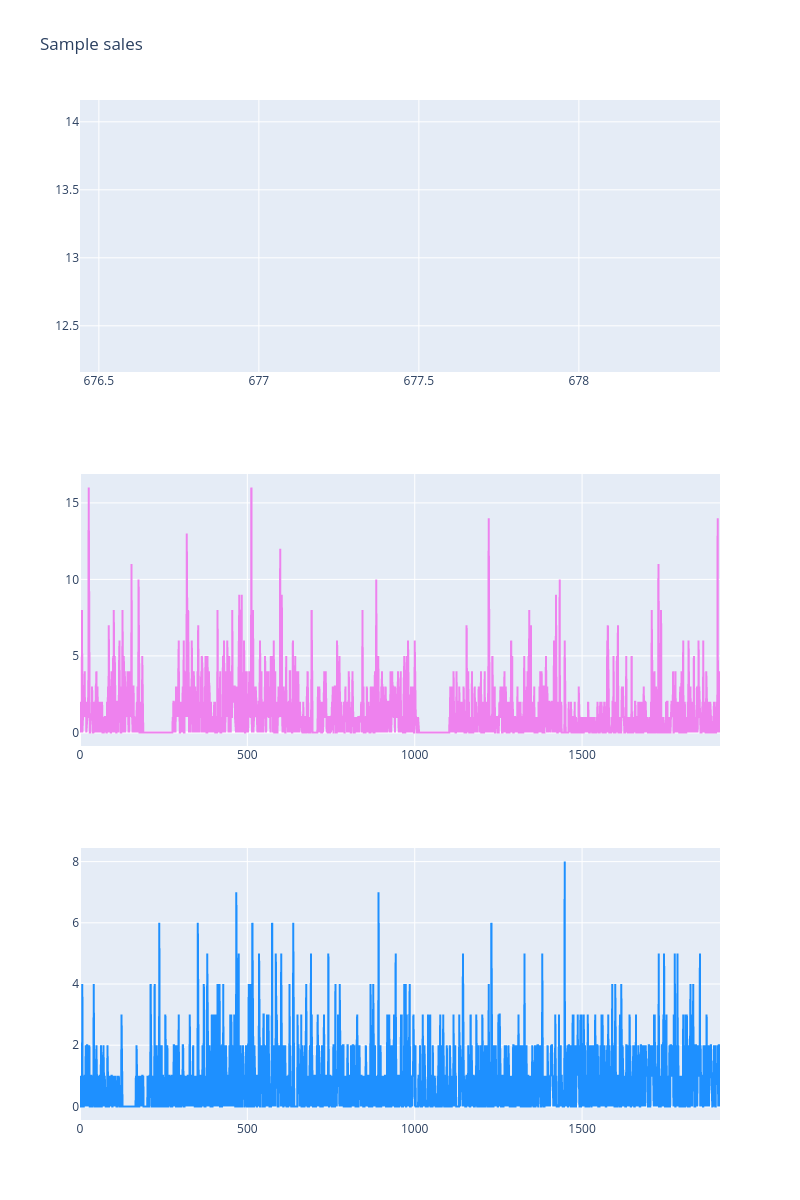
\includegraphics[width=\textwidth,height=14cm]{Outputs/4.png}
\end{figure}
\ \\
این نمونه‌ها، شامل رکورد فروش‌های فروشگاه‌هایی است که به‌طور تصادفی از مجموعه‌داده انتخاب شده است. همانطور که انتظار می‌رود، داده فروش‌ها بسیار نامنظم است، چراکه عوامل زیادی روی فروش‌های یک روز مشخص تاثیرگذار است. در روزهای مشخصی تعداد فروش‌ صفر است؛ و دلیل آن در دسترس نبودن محصول در آن روز‌هاست.
\subsection*{\lr{Denoising}}
حالا نشان خواهیم داد چگونه می‌توان نویز این فروش‌های متغیر را از بین برد، تا بتوانیم ترند‌های اساسی را استخراج کنیم. این روش موجب از دست دادن اطلاعاتی از سری‌ زمانی اصلی می‌شود، اما استخراج ویژگی‌های مشخص در جهت نشان دادن ترند‌ها در سری‌ زمانی مفید است.
\subsection*{\lr{Wavelet denoising}}
\lr{Wavelet denoising}
 یک روش برای حذف نویز اضافی از سری‌ زمانی است. این روش ضرایبی که به‌آن \lr{wavelet coefficients} می‌گویند را محسابه می‌کند. این ضرایب تعیین می‌کند که کدام بخش‌های داده را نگاه داریم (سیگنال) و کدام بخش‌ها را دور بریزیم (نویز).\\
 ما از 
 \lr{MAD}\footnote{\lr{mean absolute deviation}} 
 جهت پی‌بردن به تصادفی بودن فروش‌ها بهره می‌بریم که بر اساس آن \lr{minimum threshold}
 برای ضرایب در سری‌ زمانی تعیین می‌شود. ما ضرایبی که مقدار پایین‌تری دارند را فیلتر کرده سپس، داده فروش‌ها را بازسازی می‌کنیم. همین است!-با موفقیت نویز را از داده فروش‌ها حذف کردیم. 
\begin{latin}
\begin{lstlisting}[language=Python]
def maddest(d, axis=None):
return np.mean(np.absolute(d - np.mean(d, axis)), axis)

def denoise_signal(x, wavelet='db4', level=1):
coeff = pywt.wavedec(x, wavelet, mode="per")
sigma = (1/0.6745) * maddest(coeff[-level])

uthresh = sigma * np.sqrt(2*np.log(len(x)))
coeff[1:] = (pywt.threshold(i, value=uthresh, mode='hard') for i in coeff[1:])

return pywt.waverec(coeff, wavelet, mode='per')
\end{lstlisting}
\end{latin}
\begin{figure}[hbt!]
\centering
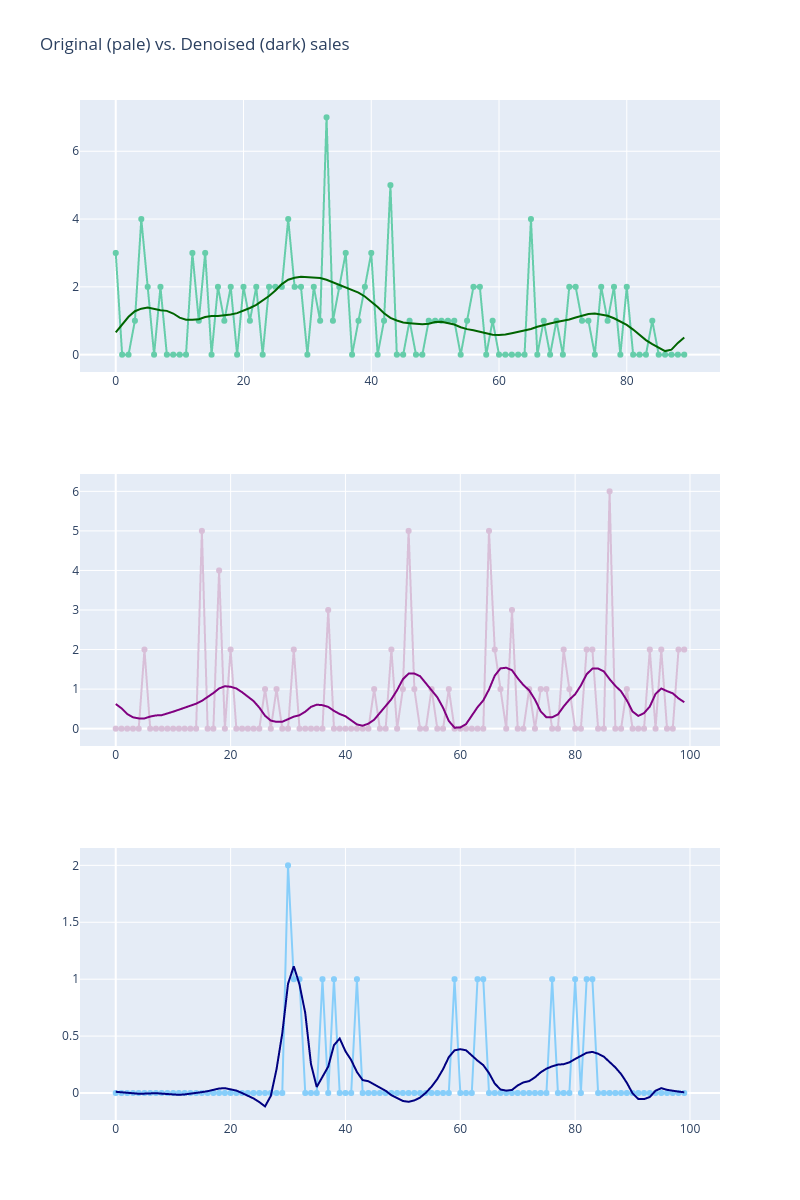
\includegraphics[width=\textwidth,height=10cm]{Outputs/6.png}
\end{figure}
\ \\
در گراف‌های بالا، \lr{lineplot}-هایی که رنگ تیره‌تر دارند، نشان‌دهنده‌ داده فروش‌های \lr{denoised} است؛ و لاین‌پلات‌هایی که رنگ روشن‌تر دارند فروش‌های اصلی را نشان می‌دهد. مشاهده می‌کنید که \lr{Wavelet denoising} قادر است با موفقیت \lr{general trend}
را در داده فروش‌ها پیدا کند. پیدا کردن این الگوها در فروش‌ها می‌تواند در تولید ویژگی‌ها برای آموزش یک مدل مفید باشد.\\
دیاگرام زیر، گراف‌ها را کنار هم نشان می‌دهد:
\begin{figure}[hbt!]
	\centering
	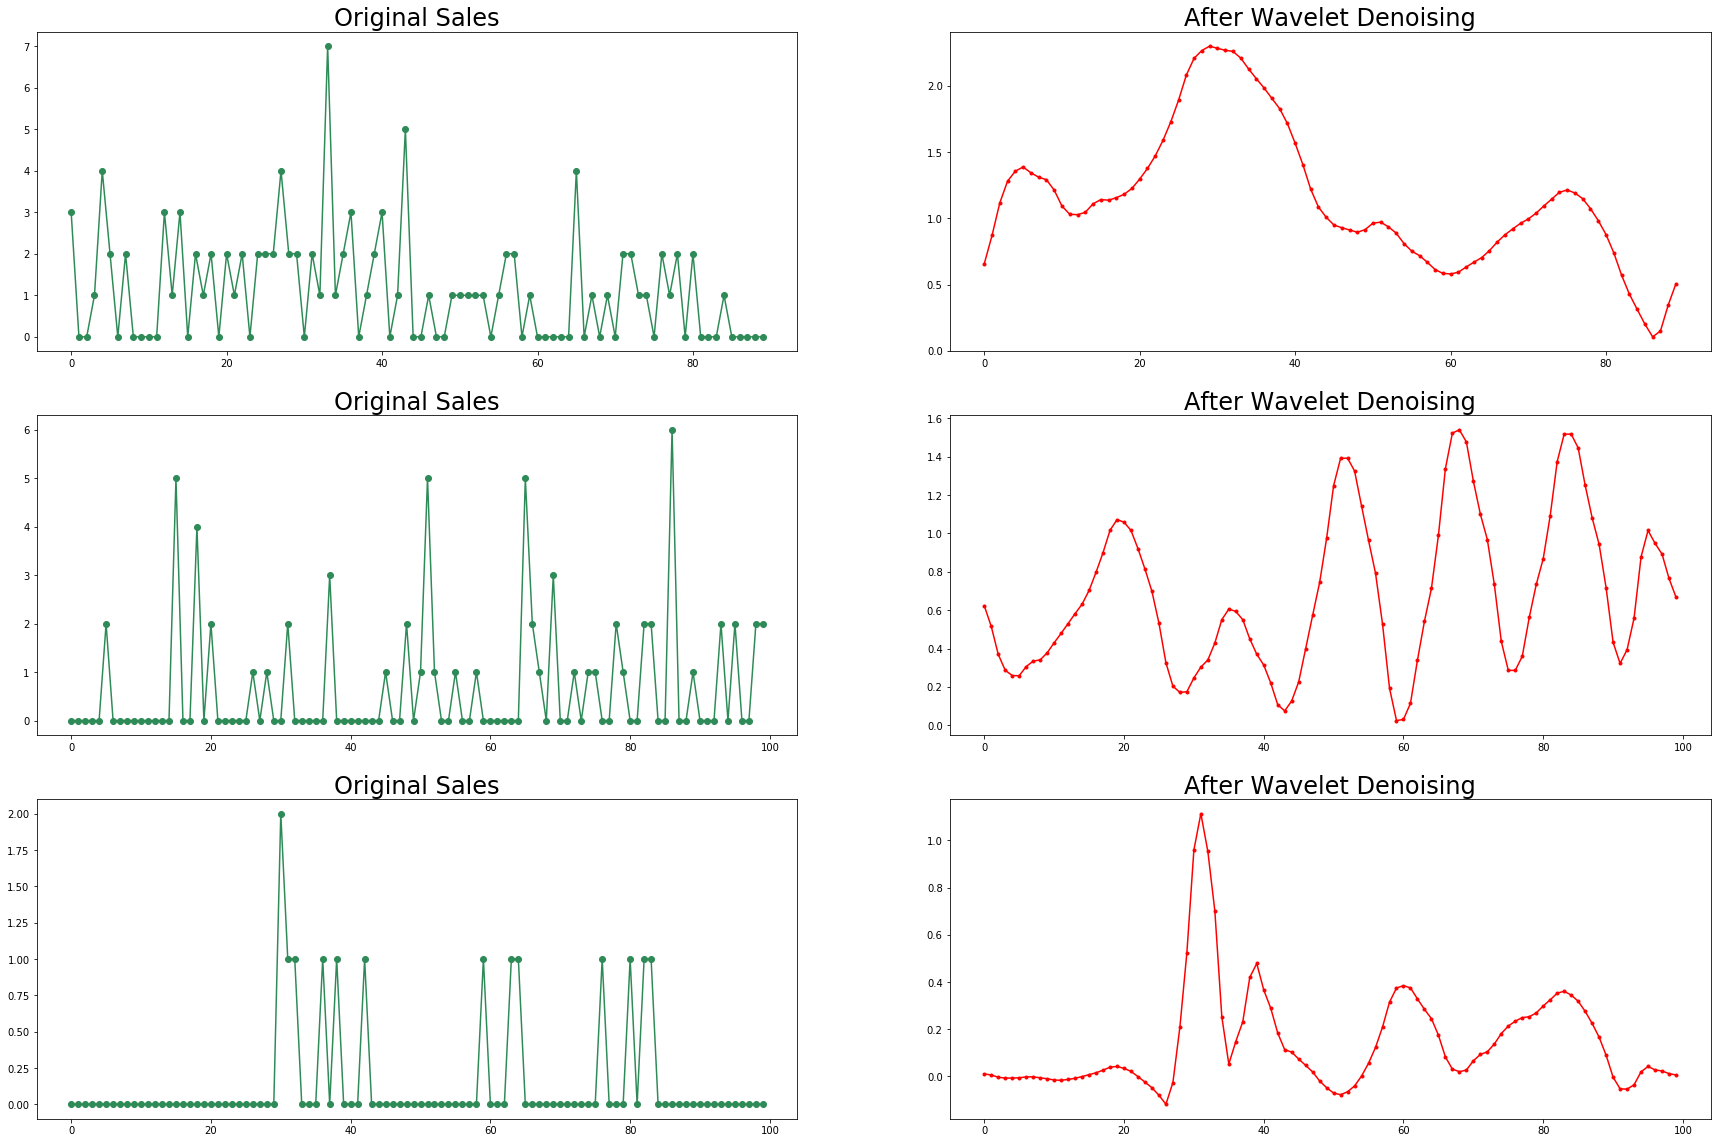
\includegraphics[width=\textwidth,height=10cm]{Outputs/8.png}
\end{figure}
\ \\
\subsection*{\lr{Average smoothing}}
\lr{Average smoothing} 
یک روش نسبتا ساده برای \lr{denoise} کردن داده سری‌ زمانی است. در این روش، ما یک پنجره با اندازه ثابت (مثلا ۱۰) در نظر می‌گیریم. ابتدا پنجره را در اول سری‌ زمانی قرار می‌دهیم (ده سطر اول) و میانه این بخش را محاسبه می‌کنیم. حال بر اساس یک گام مشخص، پنجره را تا انتهای سری‌ جلو می‌بریم. برای تمام پنجره‌ها میانه محاسبه خواهد شد؛ سپس، با میانه‌های به‌دست آمده، سری زمانی جدید ساخته می‌شود که داده‌ \lr{denoised} را تشکیل می‌دهد.
\begin{latin}
\begin{lstlisting}[language=Python]
def average_smoothing(signal, kernel_size=3, stride=1):
	sample = []
	start = 0
	end = kernel_size
	while end <= len(signal):
		start = start + stride
		end = end + stride
		sample.extend(np.ones(end - start)*np.mean(signal[start:end]))
	return np.array(sample)
\end{lstlisting}
\end{latin}
\ \\
مقایسه سیگنال‌های اصلی (کم‌رنگ) با سیگنال‌های \lr{denoised} شده (پررنگ) :
\begin{latin}
\begin{lstlisting}[language=Python]
y_a1 = average_smoothing(x_1)
y_a2 = average_smoothing(x_2)
y_a3 = average_smoothing(x_3)

fig = make_subplots(rows=3, cols=1)

fig.add_trace(
go.Scatter(x=np.arange(len(x_1)), mode='lines+markers', y=x_1, marker=dict(color="lightskyblue"), showlegend=False,
name="Original sales"),
row=1, col=1
)

fig.add_trace(
go.Scatter(x=np.arange(len(x_1)), y=y_a1, mode='lines', marker=dict(color="navy"), showlegend=False,
name="Denoised sales"),
row=1, col=1
)

fig.add_trace(
go.Scatter(x=np.arange(len(x_2)), mode='lines+markers', y=x_2, marker=dict(color="thistle"), showlegend=False),
row=2, col=1
)

fig.add_trace(
go.Scatter(x=np.arange(len(x_2)), y=y_a2, mode='lines', marker=dict(color="indigo"), showlegend=False),
row=2, col=1
)

fig.add_trace(
go.Scatter(x=np.arange(len(x_3)), mode='lines+markers', y=x_3, marker=dict(color="mediumaquamarine"), showlegend=False),
row=3, col=1
)

fig.add_trace(
go.Scatter(x=np.arange(len(x_3)), y=y_a3, mode='lines', marker=dict(color="darkgreen"), showlegend=False),
row=3, col=1
)

fig.update_layout(height=1200, width=800, title_text="Original (pale) vs. Denoised (dark) signals")
fig.show()
\end{lstlisting}
\end{latin}
\pagebreak
\begin{figure}[hbt!]
	\centering
	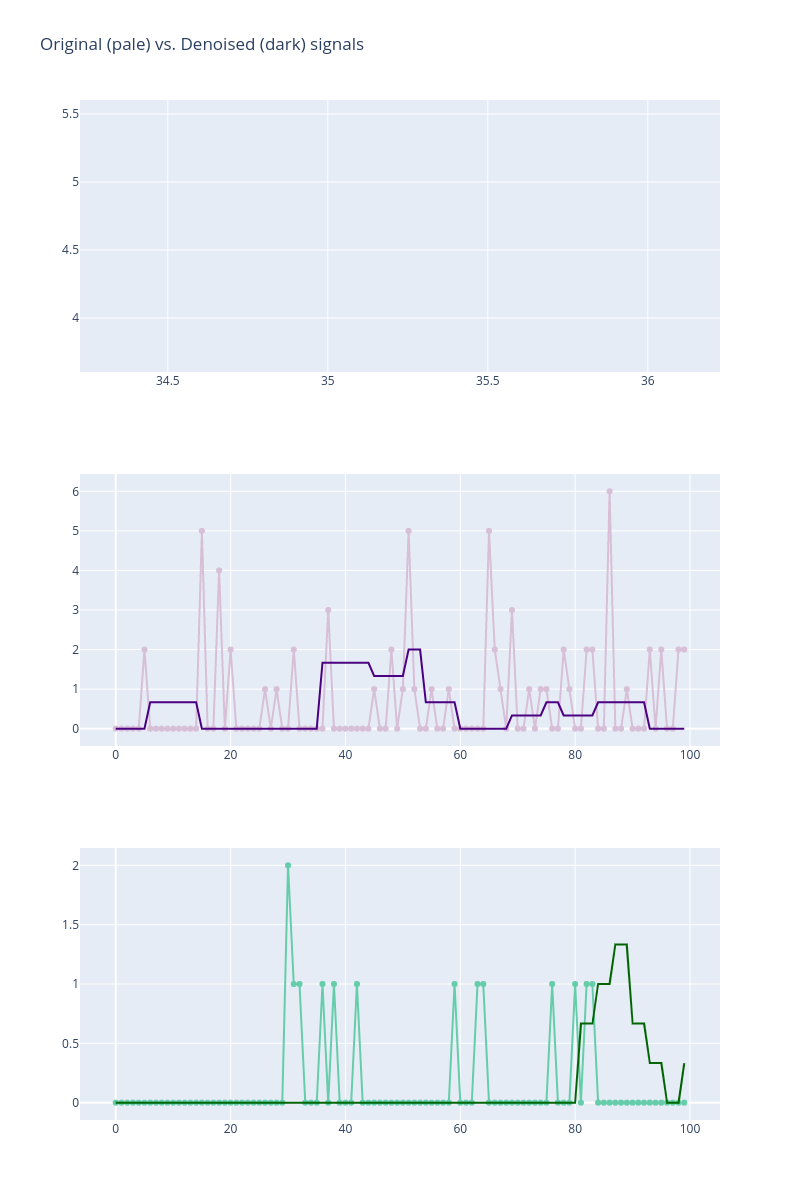
\includegraphics[width=\textwidth,height=10cm]{Outputs/10.png}
\end{figure}
\ \\
می‌توان دید \lr{average smoothing} به‌اندازه \lr{Wavelet denoising}، در پیدا کردن ترندهای ماکروسکوپی و الگوها موثر نیست. بیشتر نویز داده حتی بعد \lr{denoise} کردن پایدار است. از این رو، \lr{Wavelet denoising} به وضوح برای پیدا کردن ترندها بهتر است؛ هر چند، \lr{average smoothing} و \lr{rolling mean} هم برای محاسبه ویژگی‌های مفید، قابل استفاده است.\\
دیاگرام زیر این گراف‌ها را در کنار هم نشان می‌دهد:
\begin{latin}
\begin{lstlisting}[language=Python]
fig, ax = plt.subplots(nrows=3, ncols=2, figsize=(30, 20))

ax[0, 0].plot(x_1, color='seagreen', marker='o') 
ax[0, 0].set_title('Original Sales', fontsize=24)
ax[0, 1].plot(y_a1, color='red', marker='.') 
ax[0, 1].set_title('After Wavelet Denoising', fontsize=24)

ax[1, 0].plot(x_2, color='seagreen', marker='o') 
ax[1, 0].set_title('Original Sales', fontsize=24)
ax[1, 1].plot(y_a2, color='red', marker='.') 
ax[1, 1].set_title('After Wavelet Denoising', fontsize=24)

ax[2, 0].plot(x_3, color='seagreen', marker='o') 
ax[2, 0].set_title('Original Sales', fontsize=24)
ax[2, 1].plot(y_a3, color='red', marker='.') 
ax[2, 1].set_title('After Wavelet Denoising', fontsize=24)

plt.show()
\end{lstlisting}
\end{latin}
\begin{figure}[hbt!]
	\centering
	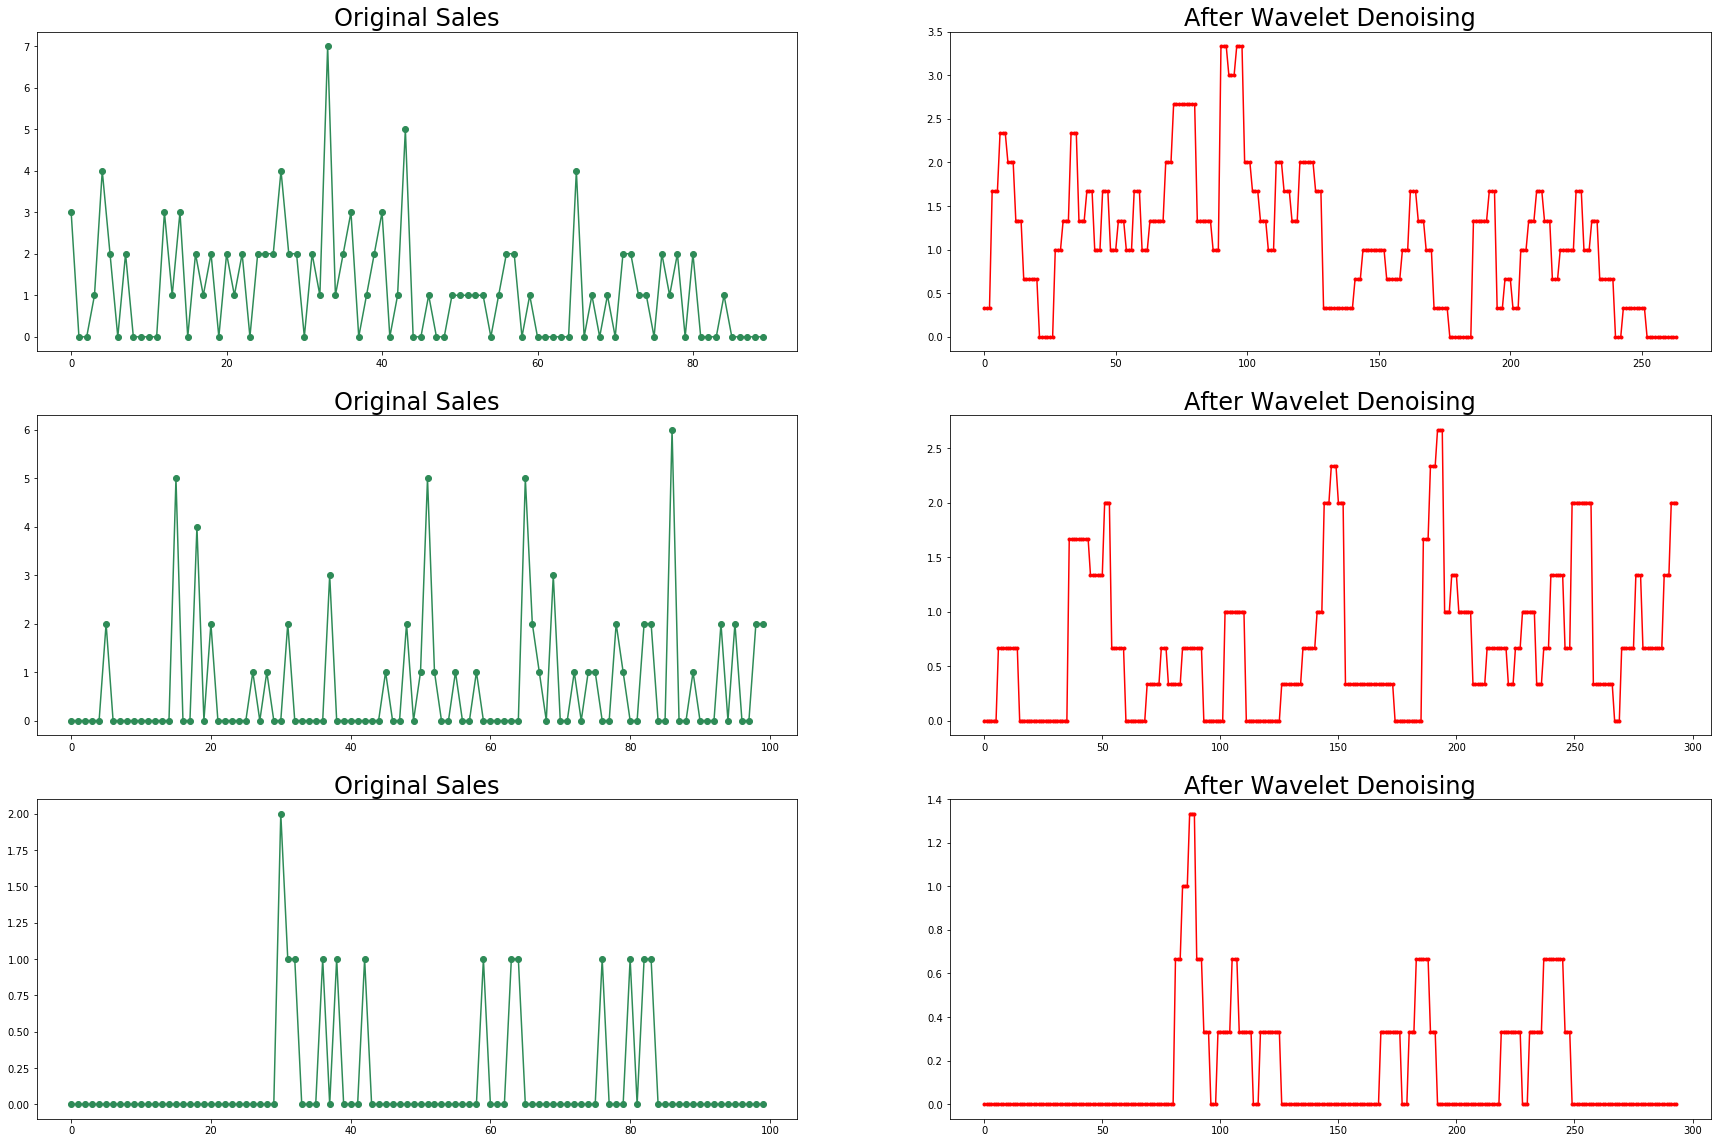
\includegraphics[width=\textwidth,height=10cm]{Outputs/11.png}
\end{figure}
\ \\
\subsection*{فروشگاه‌ها و ایالت‌ها}
حالا برای کسب اطلاعات مفید، می‌خواهیم نگاهی به فروش‌ها در فروشگاه‌ها و ایالت‌های متفاوت بی‌اندازیم.
\subsubsection*{\lr{Rolling Average Price vs. Time (per store)}}
\begin{latin}
\begin{lstlisting}[language=Python]
past_sales = sales_train_val.set_index('id')[d_cols] \
.T \
.merge(calendar.set_index('d')['date'],
left_index=True,
right_index=True,
validate='1:1') \
.set_index('date')

store_list = selling_prices['store_id'].unique()
means = []
fig = go.Figure()
for s in store_list:
	store_items = [c for c in past_sales.columns if s in c]
	data = past_sales[store_items].sum(axis=1).rolling(90).mean()
	means.append(np.mean(past_sales[store_items].sum(axis=1)))
	fig.add_trace(go.Scatter(x=np.arange(len(data)), y=data, name=s))

fig.update_layout(yaxis_title="Sales", xaxis_title="Time", title="Rolling Average Sales vs. Time (per store)")
\end{lstlisting}
\end{latin}
\begin{figure}[hbt!]
	\centering
	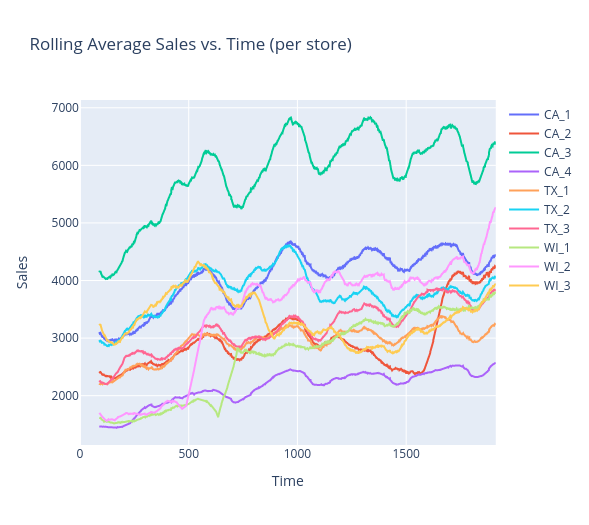
\includegraphics[width=\textwidth,height=7cm]{Outputs/12.png}
\end{figure}
\ \\
در گراف بالا، ما \lr{rolling sales} را برای تمام فروشگاه‌ها ترسیم کرده‌ایم. تقریباً  تمام منحنی‌های فروش در پلات بالا، دارای نوسان خطی هستند. فروش‌ها مانند یک موج سینوسی با میانگین مشخص در نوسان هستند، اما این میانگین ترند خطی رو به‌بالا دارد. این نشان می‌دهد فروش‌ها هر چند ماه با سطح بالاتر نوسان می‌کنند.\\
این ترند یادآور \lr{business cycle} است، که در آن نوسانات کوتاه‌مدت وجود دارد اما دارای یک رشد خطی در بلند‌مدت است. شاید چنین ترندهای مقیاس‌پایین، در سطح فروشگاه‌ها، باعث درک بهتر ترندهای \lr{macroeconomic} شوند. در پایین نمایشی از این مفاهیم را مشاهده می‌کنید:
\begin{figure}[hbt!]
	\centering
	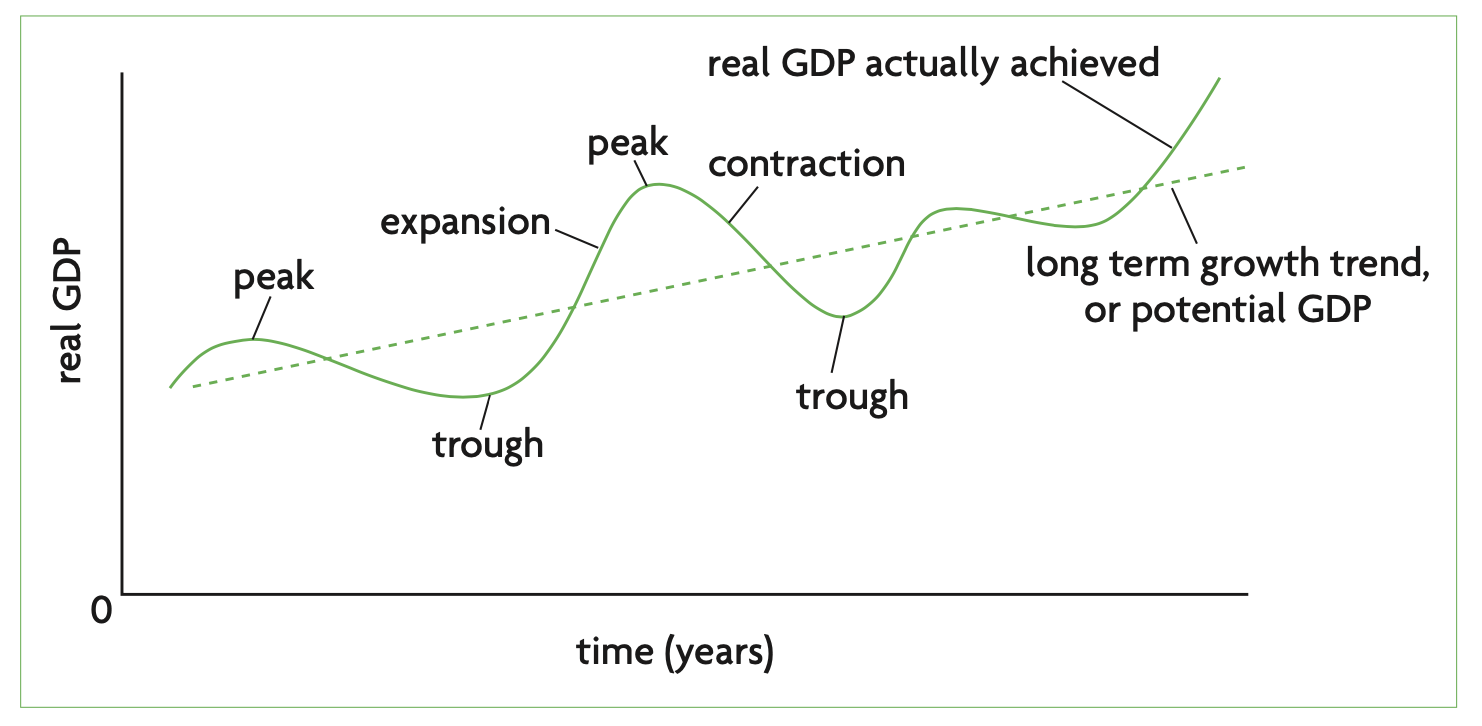
\includegraphics[width=\textwidth,height=5cm]{Outputs/o1.png}
\end{figure}
\ \\
\begin{latin}
\begin{lstlisting}[language=Python]
fig = go.Figure()

for i, s in enumerate(store_list):
	store_items = [c for c in past_sales.columns if s in c]
	data = past_sales[store_items].sum(axis=1).rolling(90).mean()
	fig.add_trace(go.Box(x=[s]*len(data), y=data, name=s))

fig.update_layout(yaxis_title="Sales", xaxis_title="Time", title="Rolling Average Sales vs. Store name ")
\end{lstlisting}
\end{latin}
\begin{figure}[hbt!]
	\centering
	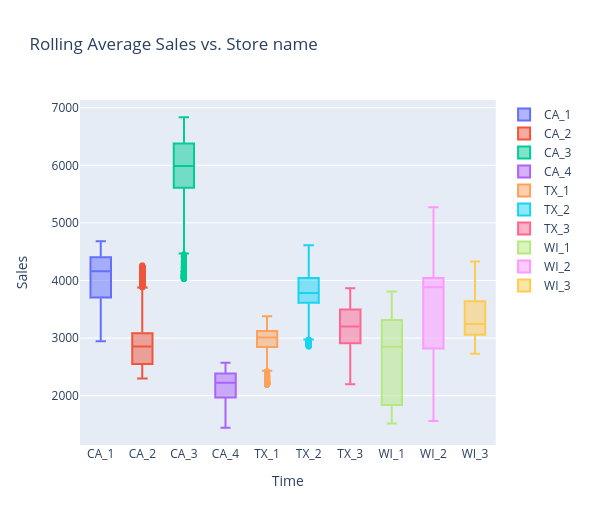
\includegraphics[width=\textwidth,height=7cm]{Outputs/13.png}
\end{figure}
\ \\
پلات بالا توزیع فروش‌ها برای هر فروشگاه در مجموعه‌داده‌ را نشان می‌دهد. فروشگاه‌هایی که در کالیفرنیا هستند، به‌نظر دارای بیشترین واریانس در فروش‌ها هستند که نشان می‌دهد بعضی مکان‌ها در کالیفرنیا به‌طور قابل ملاحضه‌ بیشتر از مکان‌های دیگر رشد دارند. از دید دیگر، فروش‌های ویسکانسین و تگزاس به‌نظر در میان خودشان بدون واریانس زیاد، ثابت‌قدم هستند. این می‌تواند نشان‌دهنده توسعه یک‌دست در این ایالت‌ها باشد. علاوه بر این، کالیفرنیا دارای بیشتر میانگین فروش‌ها است.
\begin{latin}
\begin{lstlisting}[language=Python]
df = pd.DataFrame(np.transpose([means, store_list]))
df.columns = ["Mean sales", "Store name"]
px.bar(df, y="Mean sales", x="Store name", color="Store name", title="Mean sales vs. Store name")
\end{lstlisting}
\end{latin}
\pagebreak
\begin{figure}[hbt!]
	\centering
	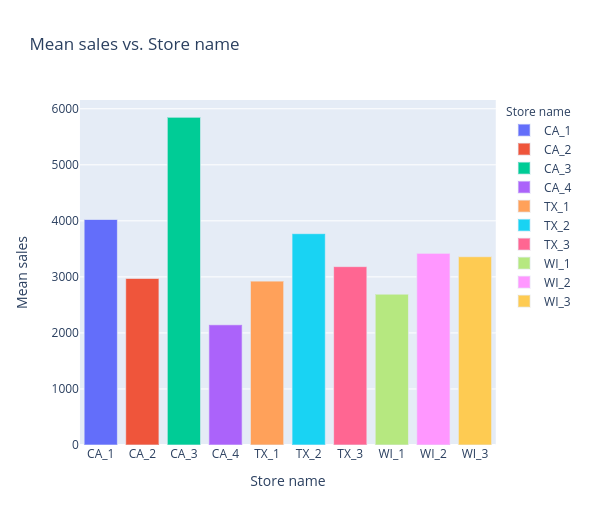
\includegraphics[width=\textwidth,height=7cm]{Outputs/14.png}
\end{figure}
\ \\
\section{مدلینگ}
در این بخش از روش‌های مختلفی برای پیش‌بینی سری زمانی استفاده برده‌ایم. این روش‌ها عبارت‌اند از:
\begin{flushleft}
\begin{latin}
\begin{itemize}
\item
\lr{naive approach}
\item
\lr{moving average}
\item
\lr{Holt linear}
\item
\lr{exponential smoothing}
\item
\lr{ARIMA}
\item
\lr{Prophet}
\end{itemize}
\end{latin}
\end{flushleft}
\subsection*{\lr{Train/Val split}}
ابتدا دو مجموعه‌داده کوچک آموزشی و آزمایشی را جدا می‌کنیم تا مدل‌ها را ارزیابی کنیم. فروش‌های ۳۰ روز پایانی برای داده آزمایشی و فروش‌های ۷۰ روز قبل‌تر برای داده‌ آموزشی انتخاب شده است. باید فروش‌های داده‌ آزمایشی را با استفاده از داده آموزشی پیش‌بینی کنیم.
\begin{latin}
\begin{lstlisting}[language=Python]
train_dataset = sales_train_val[d_cols[-100:-30]]
val_dataset = sales_train_val[d_cols[-30:]]
\end{lstlisting}
\end{latin}
\ \\
در پلات پایین، فروش‌های سه نقطه نمونه را مشاهده می‌کنید. ما از این نمونه‌ها برای نشان دادن عملکرد مدل‌ها بهره خواهیم برد.
\begin{latin}
\begin{lstlisting}[language=Python]
fig = make_subplots(rows=3, cols=1)

fig.add_trace(
go.Scatter(x=np.arange(70), mode='lines', y=train_dataset.loc[0].values, marker=dict(color="dodgerblue"), showlegend=False,
name="Original signal"),
row=1, col=1
)

fig.add_trace(
go.Scatter(x=np.arange(70, 100), y=val_dataset.loc[0].values, mode='lines', marker=dict(color="darkorange"), showlegend=False,
name="Denoised signal"),
row=1, col=1
)

fig.add_trace(
go.Scatter(x=np.arange(70), mode='lines', y=train_dataset.loc[1].values, marker=dict(color="dodgerblue"), showlegend=False),
row=2, col=1
)

fig.add_trace(
go.Scatter(x=np.arange(70, 100), y=val_dataset.loc[1].values, mode='lines', marker=dict(color="darkorange"), showlegend=False),
row=2, col=1
)

fig.add_trace(
go.Scatter(x=np.arange(70), mode='lines', y=train_dataset.loc[2].values, marker=dict(color="dodgerblue"), showlegend=False),
row=3, col=1
)

fig.add_trace(
go.Scatter(x=np.arange(70, 100), y=val_dataset.loc[2].values, mode='lines', marker=dict(color="darkorange"), showlegend=False),
row=3, col=1
)

fig.update_layout(height=1200, width=800, title_text="Train (blue) vs. Validation (orange) sales")
fig.show()
\end{lstlisting}
\end{latin}
\pagebreak
\begin{figure}[hbt!]
	\centering
	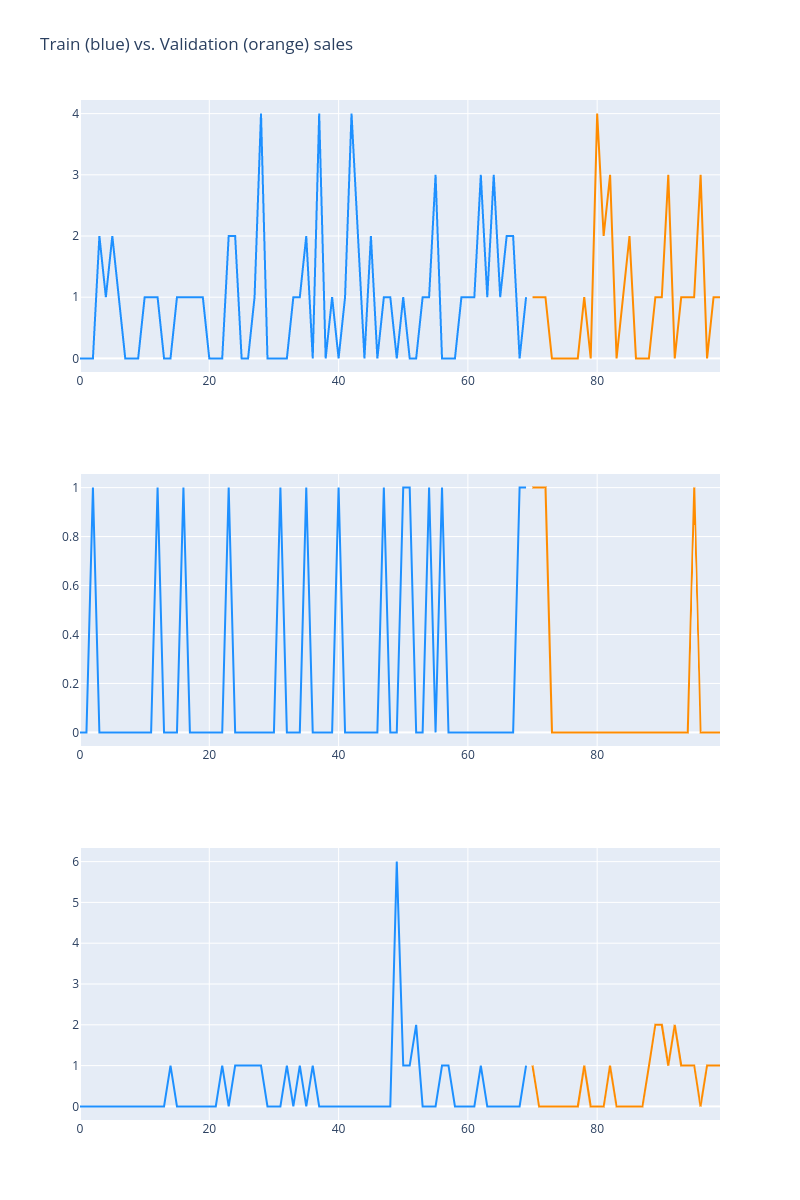
\includegraphics[width=\textwidth,height=12cm]{Outputs/25.png}
\end{figure}
\ \\
\subsection*{\lr{Naive approach}}
رویکرد اول رویکرد ساده‌یی است که فروش‌های روز بعد را برابر فروش‌های امروز قرار می‌دهد. این مدل را می‌توان به‌صورت زیر خلاصه‌سازی کرد:
\begin{figure}[hbt!]
	\centering
	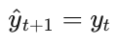
\includegraphics[width=2cm,height=1cm]{Outputs/e2.png}
\end{figure}
\ \\
بیایید ‌عملکرد مدل \lr{naive approach} را بر روی نمونه‌ها بررسی کنیم: 
\begin{latin}
\begin{lstlisting}[language=Python]
predictions = []
for i in range(len(val_dataset.columns)):
	if i == 0:
		predictions.append(train_dataset[train_dataset.columns[-1]].values)
	else:
		predictions.append(val_dataset[val_dataset.columns[i-1]].values)

predictions = np.transpose(np.array([row.tolist() for row in predictions]))
error_naive = np.linalg.norm(predictions[:3] - val_dataset.values[:3])/len(predictions[0])
\end{lstlisting}
\end{latin}
\begin{latin}
\begin{lstlisting}[language=Python]
pred_1 = predictions[0]
pred_2 = predictions[1]
pred_3 = predictions[2]

fig = make_subplots(rows=3, cols=1)

fig.add_trace(
go.Scatter(x=np.arange(70), mode='lines', y=train_dataset.loc[0].values, marker=dict(color="dodgerblue"),
name="Train"),
row=1, col=1
)

fig.add_trace(
go.Scatter(x=np.arange(70, 100), y=val_dataset.loc[0].values, mode='lines', marker=dict(color="darkorange"),
name="Val"),
row=1, col=1
)

fig.add_trace(
go.Scatter(x=np.arange(70, 100), y=pred_1, mode='lines', marker=dict(color="seagreen"),
name="Pred"),
row=1, col=1
)

fig.add_trace(
go.Scatter(x=np.arange(70), mode='lines', y=train_dataset.loc[1].values, marker=dict(color="dodgerblue"), showlegend=False),
row=2, col=1
)

fig.add_trace(
go.Scatter(x=np.arange(70, 100), y=val_dataset.loc[1].values, mode='lines', marker=dict(color="darkorange"), showlegend=False),
row=2, col=1
)

fig.add_trace(
go.Scatter(x=np.arange(70, 100), y=pred_2, mode='lines', marker=dict(color="seagreen"), showlegend=False,
name="Denoised signal"),
row=2, col=1
)

fig.add_trace(
go.Scatter(x=np.arange(70), mode='lines', y=train_dataset.loc[2].values, marker=dict(color="dodgerblue"), showlegend=False),
row=3, col=1
)

fig.add_trace(
go.Scatter(x=np.arange(70, 100), y=val_dataset.loc[2].values, mode='lines', marker=dict(color="darkorange"), showlegend=False),
row=3, col=1
)

fig.add_trace(
go.Scatter(x=np.arange(70, 100), y=pred_3, mode='lines', marker=dict(color="seagreen"), showlegend=False,
name="Denoised signal"),
row=3, col=1
)

fig.update_layout(height=1200, width=800, title_text="Naive approach")
fig.show()
\end{lstlisting}
\end{latin}
\begin{figure}[hbt!]
	\centering
	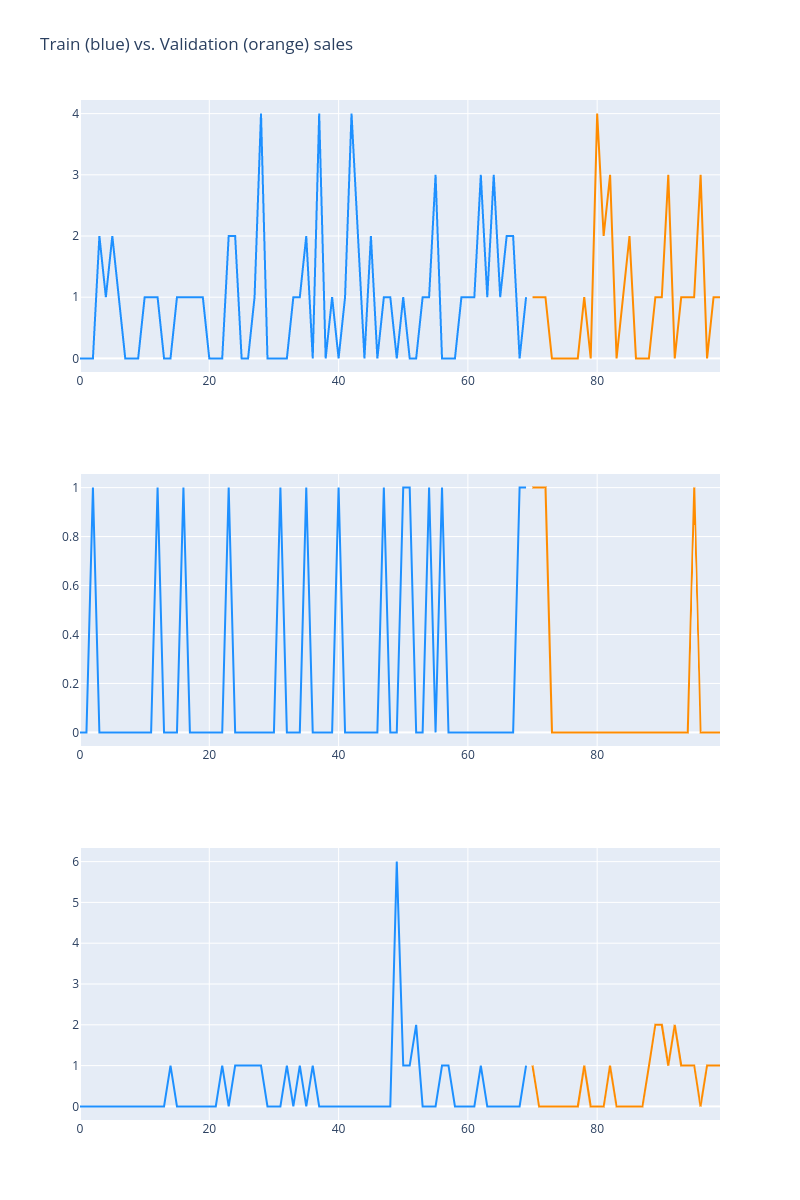
\includegraphics[width=\textwidth,height=12cm]{Outputs/25.png}
\end{figure}
\ \\
مشاهده می‌کنید، پیش‌بینی‌های انجام شده توسط رویکرد ساده دقیق نیست که از این مدل ساده‌ همین انتظار می‌رود.
\subsection*{\lr{Moving average}}
روش \lr{moving average} پیچیده‌تراز روش ساده بالاست. این روش، میانگین فروش‌های ۳۰-یا هر چند- روز را به‌عنوان فروش‌های روز بعد محاسبه می‌کند. در این روش ۳۰ گام زمانی در نظر گرفته می‌شود، به این علت کمتر به نوسانات کوتاه مدت تمایل نشان می‌دهد. این مدل را می‌توان به‌صورت زیر خلاصه‌سازی کرد:
\begin{figure}[hbt!]
	\centering
	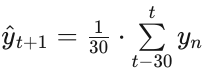
\includegraphics[width=5cm,height=1cm]{Outputs/e1.png}
\end{figure}
\ \\
بیایید ‌عملکرد مدل \lr{moving average} را بر روی نمونه‌ها بررسی کنیم: 
\begin{latin}
\begin{lstlisting}[language=Python]
predictions = []
for i in range(len(val_dataset.columns)):
	if i == 0:
		predictions.append(np.mean(train_dataset[train_dataset.columns[-30:]].values, axis=1))
	if i < 31 and i > 0:
		predictions.append(0.5 * (np.mean(train_dataset[train_dataset.columns[-30+i:]].values, axis=1 + \ np.mean(predictions[:i], axis=0)))
	if i > 31:
		predictions.append(np.mean([predictions[:i]], axis=1))

predictions = np.transpose(np.array([row.tolist() for row in predictions]))
error_avg = np.linalg.norm(predictions[:3] - val_dataset.values[:3])/len(predictions[0])
\end{lstlisting}
\end{latin}
\begin{latin}
\begin{lstlisting}[language=Python]
pred_1 = predictions[0]
pred_2 = predictions[1]
pred_3 = predictions[2]

fig = make_subplots(rows=3, cols=1)

fig.add_trace(
go.Scatter(x=np.arange(70), mode='lines', y=train_dataset.loc[0].values, marker=dict(color="dodgerblue"),
name="Train"),
row=1, col=1
)

fig.add_trace(
go.Scatter(x=np.arange(70, 100), y=val_dataset.loc[0].values, mode='lines', marker=dict(color="darkorange"),
name="Val"),
row=1, col=1
)

fig.add_trace(
go.Scatter(x=np.arange(70, 100), y=pred_1, mode='lines', marker=dict(color="seagreen"),
name="Pred"),
row=1, col=1
)

fig.add_trace(
go.Scatter(x=np.arange(70), mode='lines', y=train_dataset.loc[1].values, marker=dict(color="dodgerblue"), showlegend=False),
row=2, col=1
)

fig.add_trace(
go.Scatter(x=np.arange(70, 100), y=val_dataset.loc[1].values, mode='lines', marker=dict(color="darkorange"), showlegend=False),
row=2, col=1
)

fig.add_trace(
go.Scatter(x=np.arange(70, 100), y=pred_2, mode='lines', marker=dict(color="seagreen"), showlegend=False,
name="Denoised signal"),
row=2, col=1
)

fig.add_trace(
go.Scatter(x=np.arange(70), mode='lines', y=train_dataset.loc[2].values, marker=dict(color="dodgerblue"), showlegend=False),
row=3, col=1
)

fig.add_trace(
go.Scatter(x=np.arange(70, 100), y=val_dataset.loc[2].values, mode='lines', marker=dict(color="darkorange"), showlegend=False),
row=3, col=1
)

fig.add_trace(
go.Scatter(x=np.arange(70, 100), y=pred_3, mode='lines', marker=dict(color="seagreen"), showlegend=False,
name="Denoised signal"),
row=3, col=1
)

fig.update_layout(height=1200, width=800, title_text="Moving average")
fig.show()
\end{lstlisting}
\end{latin}
\pagebreak
\begin{figure}[hbt!]
	\centering
	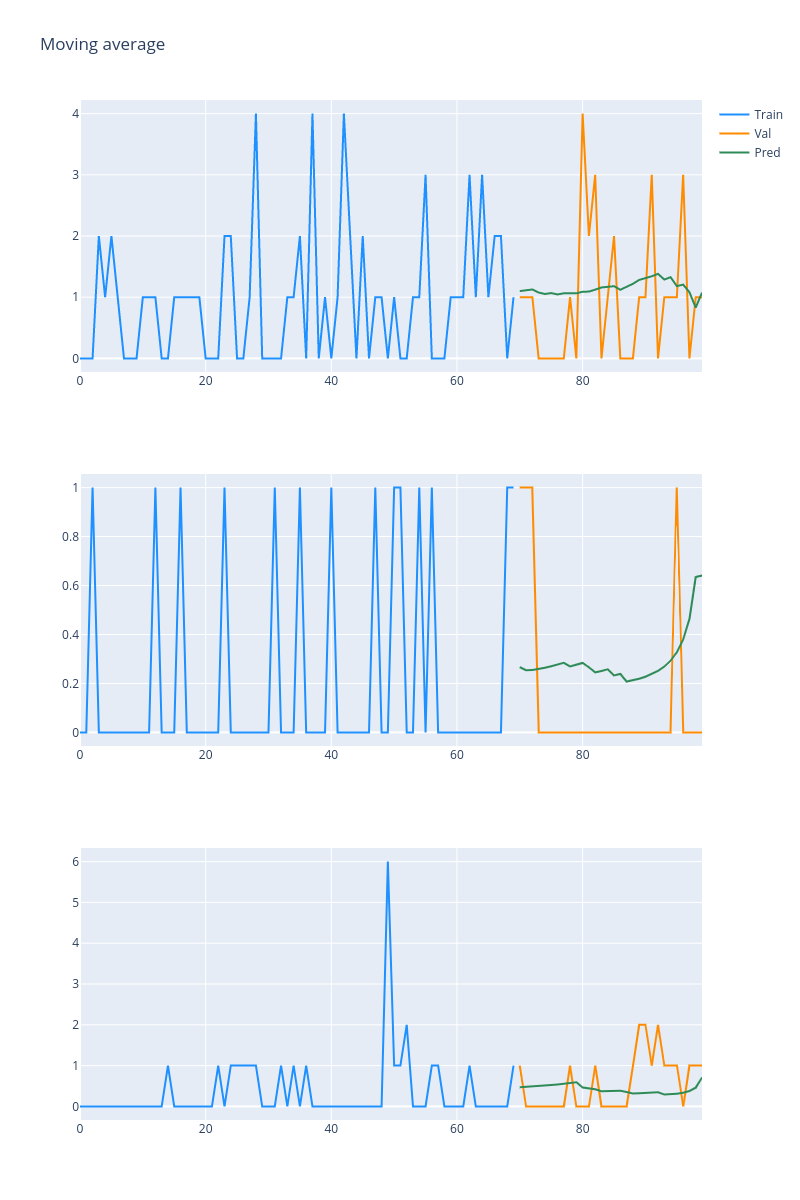
\includegraphics[width=\textwidth,height=12cm]{Outputs/29.png}
\end{figure}
\ \\
‌می‌توان دید این مدل بهتر از روش ساده عمل می‌کند و کمتر مستعد پذیرش نوسان‌های روزانه فروش‌ها است. مدل \lr{moving average} ترندها را با دقت اندکی بیشتر پیدا می‌کند. هر چند توانایی پیدا کردن ترندهای مهم را ندارد.
\subsection*{\lr{Holt linear}}
این روش کاملا متفاوت با دو روش اول است. \lr{Holt linear} تلاش می‌کند ترند‌های سطح بالا را با بهره بردن از یک تابع خطی شناسایی کند. این روش را می‌توان به‌صورت زیر خلاصه سازی کرد:
\begin{figure}[hbt!]
	\centering
	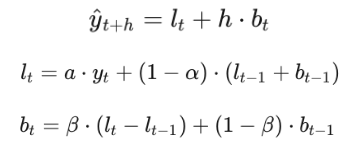
\includegraphics[width=5cm,height=3cm]{Outputs/e3.png}
\end{figure}
\ \\
در معادله‌های بالا، آلفا و بتا ثابت‌هایی‌ هستند که قابل تغییر است. \lr{l\textsubscript{t}} نشان‌دهنده‌ مقدار سطح و  \lr{b\textsubscript{t}} نشان‌دهنده مقدار ترند است. مقدار ترند برابر شیب تابع پیش‌بینی خطی است و مقدار سطح، نقطه تلاقی محور عمودی و تابع پیش‌بینی خطی است. شیب و نقطه تلاقی به‌صورت مداوم با معادله دوم و سوم به‌روز می‌شوند. در پایان، از شیب و نقطه تلاقی برای پیش‌بینی  \lr{l\textsubscript{t+1}} (در معادله اول) استفاده می‌شود. در این معادله \lr{h} تعداد گام‌های زمانی بعد از گام زمانی فعلی است.\\
بیایید ‌عملکرد مدل \lr{Holt linear} را بر روی نمونه‌ها بررسی کنیم: 
\begin{latin}
\begin{lstlisting}[language=Python]
predictions = []
for row in tqdm(train_dataset[train_dataset.columns[-30:]].values[:3]):
	fit = Holt(row).fit(smoothing_level = 0.3, smoothing_slope = 0.01)
	predictions.append(fit.forecast(30))
predictions = np.array(predictions).reshape((-1, 30))
error_holt = np.linalg.norm(predictions - val_dataset.values[:len(predictions)])/len(predictions[0])
\end{lstlisting}
\end{latin}
\begin{latin}
\begin{lstlisting}[language=Python]
pred_1 = predictions[0]
pred_2 = predictions[1]
pred_3 = predictions[2]

fig = make_subplots(rows=3, cols=1)

fig.add_trace(
go.Scatter(x=np.arange(70), mode='lines', y=train_dataset.loc[0].values, marker=dict(color="dodgerblue"),
name="Train"),
row=1, col=1
)

fig.add_trace(
go.Scatter(x=np.arange(70, 100), y=val_dataset.loc[0].values, mode='lines', marker=dict(color="darkorange"),
name="Val"),
row=1, col=1
)

fig.add_trace(
go.Scatter(x=np.arange(70, 100), y=pred_1, mode='lines', marker=dict(color="seagreen"),
name="Pred"),
row=1, col=1
)

fig.add_trace(
go.Scatter(x=np.arange(70), mode='lines', y=train_dataset.loc[1].values, marker=dict(color="dodgerblue"), showlegend=False),
row=2, col=1
)

fig.add_trace(
go.Scatter(x=np.arange(70, 100), y=val_dataset.loc[1].values, mode='lines', marker=dict(color="darkorange"), showlegend=False),
row=2, col=1
)

fig.add_trace(
go.Scatter(x=np.arange(70, 100), y=pred_2, mode='lines', marker=dict(color="seagreen"), showlegend=False,
name="Denoised signal"),
row=2, col=1
)

fig.add_trace(
go.Scatter(x=np.arange(70), mode='lines', y=train_dataset.loc[2].values, marker=dict(color="dodgerblue"), showlegend=False),
row=3, col=1
)

fig.add_trace(
go.Scatter(x=np.arange(70, 100), y=val_dataset.loc[2].values, mode='lines', marker=dict(color="darkorange"), showlegend=False),
row=3, col=1
)

fig.add_trace(
go.Scatter(x=np.arange(70, 100), y=pred_3, mode='lines', marker=dict(color="seagreen"), showlegend=False,
name="Denoised signal"),
row=3, col=1
)

fig.update_layout(height=1200, width=800, title_text="Holt linear")
fig.show()
\end{lstlisting}
\end{latin}
\pagebreak
\begin{figure}[hbt!]
	\centering
	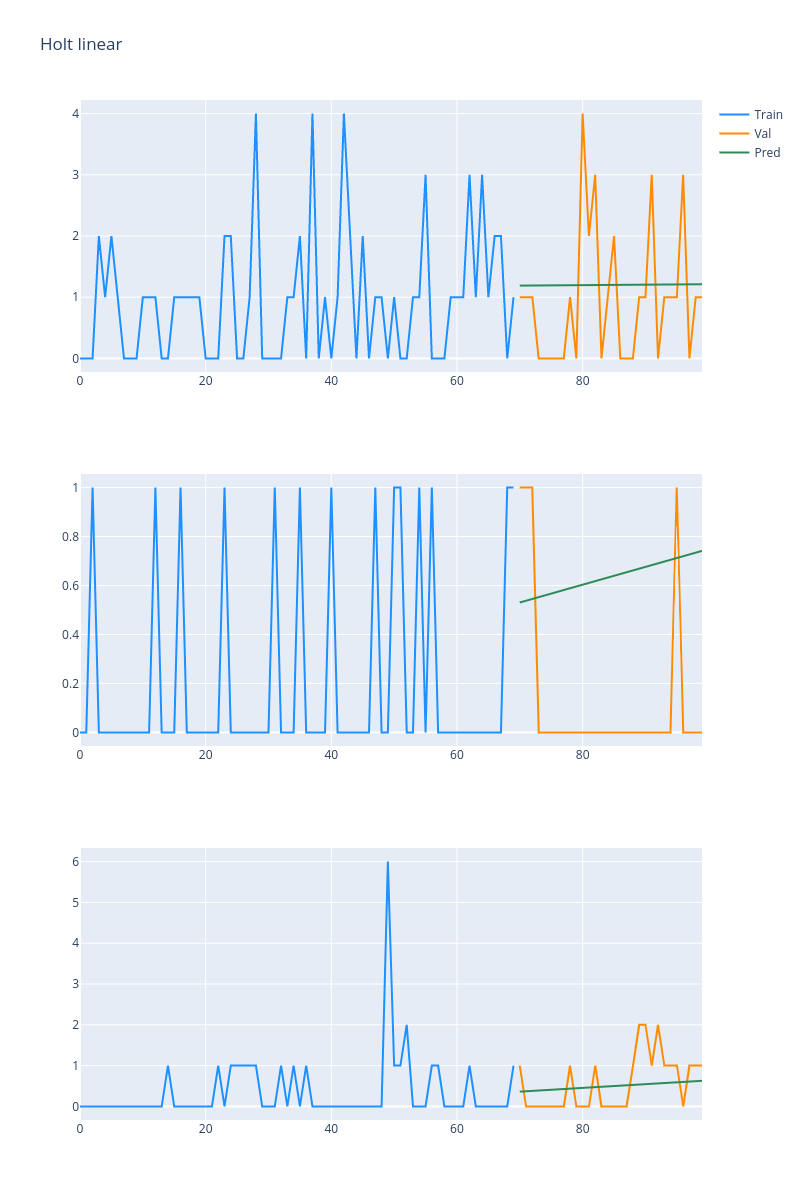
\includegraphics[width=\textwidth,height=12cm]{Outputs/31.png}
\end{figure}
\ \\
می‌توان دید \lr{Holt linear} ترندهای سطح بالا را همواره پیش‌بینی می‌کند. اما این مدل، توانایی شناسایی نوسان‌های کوتاه‌مدت را همچون روش‌های قبلی ندارد.
\subsection*{\lr{Exponential smoothing}}
در این روش از یک نوع \lr{smoothing} متفاوت استفاده می‌شود که با \lr{average smoothing} متفاوت است. گام‌های زمانی قبل از روز هدف را به‌صورت نمایی وزن‌دهی کرده و سپس با هم جمع می‌کنیم تا پیش‌بینی انجام پذیرد. این مدل می‌توان به‌صورت زیر خلاصه‌سازی کرد: 
\begin{figure}[hbt!]
	\centering
	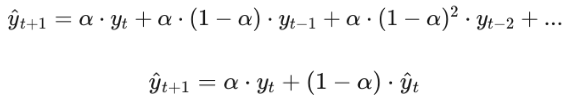
\includegraphics[width=8cm,height=2cm]{Outputs/e4.png}
\end{figure}
\ \\
در معادله‌های بالا، آلفا پارامتر \lr{smoothing} است. پیش‌بینی  \lr{y\textsubscript{t+1}} یک میانگین از بررسی‌های سری زمانی است. نرخ زوال وز‌ن‌ها با آلفا کنترل می‌شود. این روش وزن‌های متفاوتی به‌هر گام زمانی اختصاص می‌دهد (بر عکس روش میانگین). این نوع وزن‌دهی به‌ما اطمینان می‌دهد که فروش‌های اخیر اهمیت بیشتری نسبت به فروش‌های قدیمی داشته باشند.\\
حال بیایید عملکرد این مدل را بررسی کنیم:
\begin{latin}
\begin{lstlisting}[language=Python]
predictions = []
for row in tqdm(train_dataset[train_dataset.columns[-30:]].values[:3]):
	fit = ExponentialSmoothing(row, seasonal_periods=3).fit()
	predictions.append(fit.forecast(30))
predictions = np.array(predictions).reshape((-1, 30))
error_exponential = np.linalg.norm(predictions[:3] - val_dataset.values[:3])/len(predictions[0])
\end{lstlisting}
\end{latin}
\begin{latin}
\begin{lstlisting}[language=Python]
pred_1 = predictions[0]
pred_2 = predictions[1]
pred_3 = predictions[2]

fig = make_subplots(rows=3, cols=1)

fig.add_trace(
go.Scatter(x=np.arange(70), mode='lines', y=train_dataset.loc[0].values, marker=dict(color="dodgerblue"),
name="Train"),
row=1, col=1
)

fig.add_trace(
go.Scatter(x=np.arange(70, 100), y=val_dataset.loc[0].values, mode='lines', marker=dict(color="darkorange"),
name="Val"),
row=1, col=1
)

fig.add_trace(
go.Scatter(x=np.arange(70, 100), y=pred_1, mode='lines', marker=dict(color="seagreen"),
name="Pred"),
row=1, col=1
)

fig.add_trace(
go.Scatter(x=np.arange(70), mode='lines', y=train_dataset.loc[1].values, marker=dict(color="dodgerblue"), showlegend=False),
row=2, col=1
)

fig.add_trace(
go.Scatter(x=np.arange(70, 100), y=val_dataset.loc[1].values, mode='lines', marker=dict(color="darkorange"), showlegend=False),
row=2, col=1
)

fig.add_trace(
go.Scatter(x=np.arange(70, 100), y=pred_2, mode='lines', marker=dict(color="seagreen"), showlegend=False,
name="Denoised signal"),
row=2, col=1
)

fig.add_trace(
go.Scatter(x=np.arange(70), mode='lines', y=train_dataset.loc[2].values, marker=dict(color="dodgerblue"), showlegend=False),
row=3, col=1
)

fig.add_trace(
go.Scatter(x=np.arange(70, 100), y=val_dataset.loc[2].values, mode='lines', marker=dict(color="darkorange"), showlegend=False),
row=3, col=1
)

fig.add_trace(
go.Scatter(x=np.arange(70, 100), y=pred_3, mode='lines', marker=dict(color="seagreen"), showlegend=False,
name="Denoised signal"),
row=3, col=1
)

fig.update_layout(height=1200, width=800, title_text="Exponential smoothing")
fig.show()
\end{lstlisting}
\end{latin}
\begin{figure}[hbt!]
	\centering
	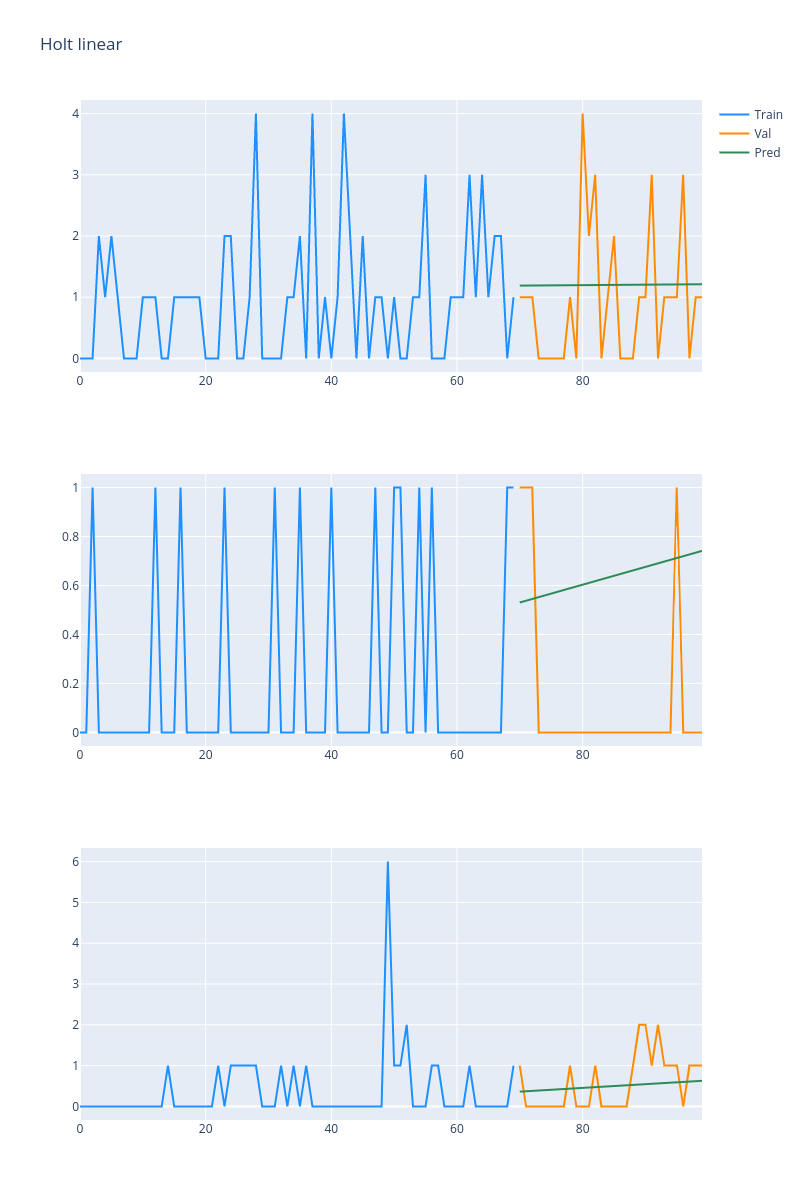
\includegraphics[width=\textwidth,height=10cm]{Outputs/31.png}
\end{figure}
\ \\
\subsection*{مدل‌های \lr{ARIMA}\footnote{\lr{Auto Regressive Integrated Moving Average}}}
\lr{ARIMA}
 در واقع یک کلاس از مدل‌هاست که یک سری زمانی را بر اساس مقادیر قبلی خود تشریح می‌کند. هر سری زمانی که الگویی داشته باشد و \lr{white noise} تصادفی نباشد با \lr{ARIMA} قابل مدل شدن است. هر مدل \lr{ARIMA} با سه شرط مشخص می‌شود: 
\begin{latin}
\begin{flushleft}
\begin{itemize}
	\item \lr{p} 
	\lr{is the order of the AR term}
	\item \lr{q
	is the order of the MA term}
	\item \lr{d
	is the number of differencing required to make the time series stationary}
\end{itemize}
\end{flushleft}
\end{latin}
\ \\
اولین گام برای ساختن یک مدل \lr{ARIMA}، ایستا کردن سری زمانی است. \lr{ar} به‌معنی \lr{auto regressive} می‌باشد و نشان می‌دهد که یک مدل رگرسیون خطی است که از خطای خودش برای پیش‌بینی استفاده می‌کند. همانطور که می‌دانید، رگرسیون خطی وقتی \lr{predictor}-ها به‌هم مرتبط نیستند بهتر عمل می‌کند. رویکرد اصلی کم کردن مقدار قبلی از مقدار فعلی‌‌ست. با توجه به پیچیدگی سری زمانی، شاید اختلاف‌های بیشتری مورد نیاز باشد. مقدار \lr{d} در این صورت برابر‌: کمینه تعداد اختلاف‌های مورد نیاز برای ایستا کردن سری زمانی است. اگر سری زمانی ایستا باشد، مقدار \lr{d} برابر صفر خواهد بود. \lr{p} برابر تعداد \lr{lag}-های \lr{Y} است که به‌عنوان \lr{predictor} استفاده خواهد شد. \lr{q} برابر تعداد خطاهای پیش‌بینی \lr{lag}-دار است که باید وارد مدل \lr{ARIMA} شود. یک مدل \lr{ARIMA} مدلی‌ست که سری زمانی در آن حداقل یک بار اختلاف‌گیری شده تا به‌وضعیت ایستا برسد. اگر ترم‌های \lr{AR} و \lr{MA} را ترکیب کنیم به معادله زیر می‌رسیم.
\begin{figure}[hbt!]
	\centering
	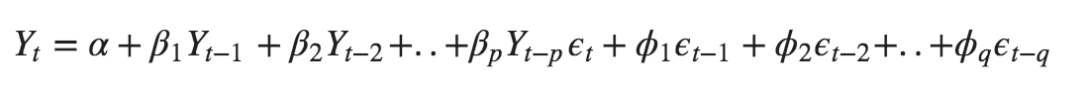
\includegraphics[width=8cm,height=1cm]{Outputs/e5.png}
\end{figure}
\ \\
\begin{latin}
\begin{flushleft}
\textbf{ARIMA model in words:}\\
Predicted Yt = Constant + Linear combination Lags of Y (upto p lags) + Linear Combination of Lagged forecast errors (upto q lags)
\end{flushleft}
\end{latin}
\ \\
حال بیایید عملکرد این مدل را بررسی کنیم:
\begin{latin}
\begin{lstlisting}[language=Python]
predictions = []
for row in tqdm(train_dataset[train_dataset.columns[-30:]].values[:3]):
	fit = sm.tsa.statespace.SARIMAX(row, seasonal_order=(0, 1, 1, 7)).fit()
	predictions.append(fit.forecast(30))
predictions = np.array(predictions).reshape((-1, 30))
error_arima = np.linalg.norm(predictions[:3] - val_dataset.values[:3])/len(predictions[0])
\end{lstlisting}
\end{latin}
\begin{latin}
\begin{lstlisting}[language=Python]
pred_1 = predictions[0]
pred_2 = predictions[1]
pred_3 = predictions[2]

fig = make_subplots(rows=3, cols=1)

fig.add_trace(
go.Scatter(x=np.arange(70), mode='lines', y=train_dataset.loc[0].values, marker=dict(color="dodgerblue"),
name="Train"),
row=1, col=1
)

fig.add_trace(
go.Scatter(x=np.arange(70, 100), y=val_dataset.loc[0].values, mode='lines', marker=dict(color="darkorange"),
name="Val"),
row=1, col=1
)

fig.add_trace(
go.Scatter(x=np.arange(70, 100), y=pred_1, mode='lines', marker=dict(color="seagreen"),
name="Pred"),
row=1, col=1
)

fig.add_trace(
go.Scatter(x=np.arange(70), mode='lines', y=train_dataset.loc[1].values, marker=dict(color="dodgerblue"), showlegend=False),
row=2, col=1
)

fig.add_trace(
go.Scatter(x=np.arange(70, 100), y=val_dataset.loc[1].values, mode='lines', marker=dict(color="darkorange"), showlegend=False),
row=2, col=1
)

fig.add_trace(
go.Scatter(x=np.arange(70, 100), y=pred_2, mode='lines', marker=dict(color="seagreen"), showlegend=False,
name="Denoised signal"),
row=2, col=1
)

fig.add_trace(
go.Scatter(x=np.arange(70), mode='lines', y=train_dataset.loc[2].values, marker=dict(color="dodgerblue"), showlegend=False),
row=3, col=1
)

fig.add_trace(
go.Scatter(x=np.arange(70, 100), y=val_dataset.loc[2].values, mode='lines', marker=dict(color="darkorange"), showlegend=False),
row=3, col=1
)

fig.add_trace(
go.Scatter(x=np.arange(70, 100), y=pred_3, mode='lines', marker=dict(color="seagreen"), showlegend=False,
name="Denoised signal"),
row=3, col=1
)

fig.update_layout(height=1200, width=800, title_text="ARIMA")
fig.show()
\end{lstlisting}
\end{latin}

\begin{figure}[hbt!]
	\centering
	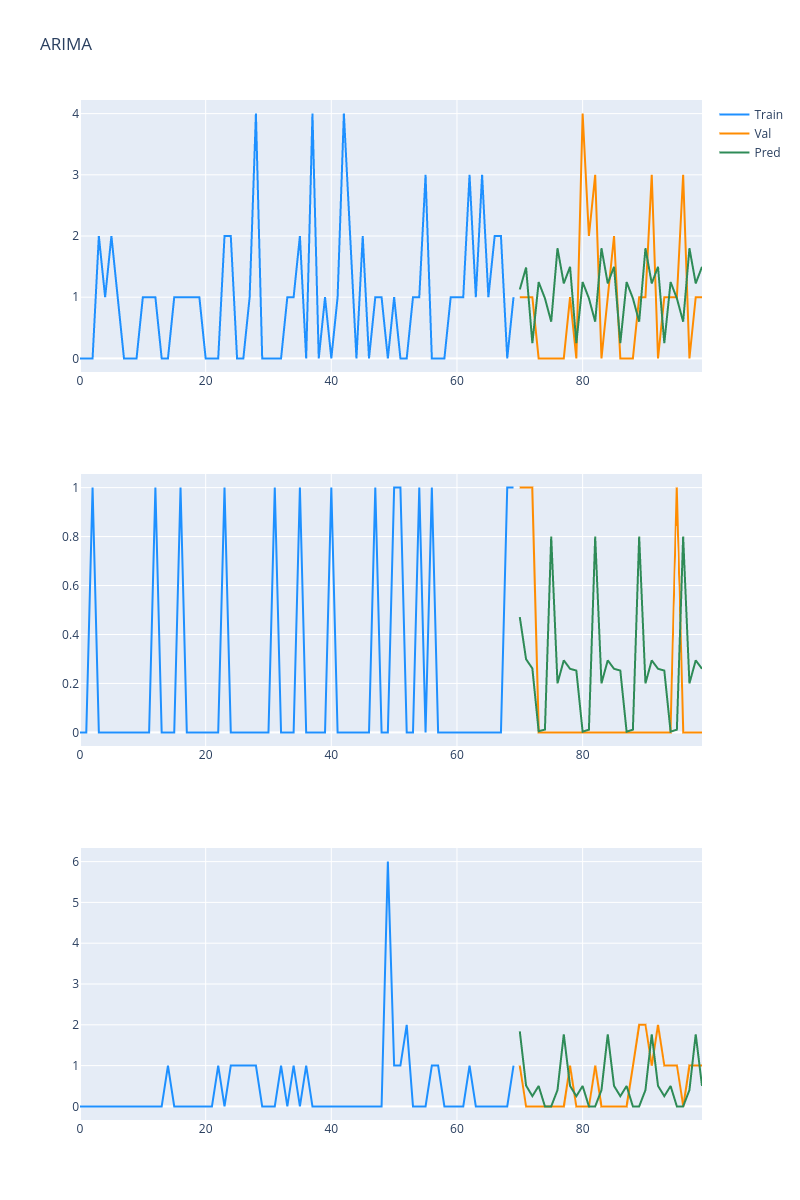
\includegraphics[width=\textwidth,height=12cm]{Outputs/36.png}
\end{figure}
\ \\
\begin{flushleft}
	\begin{latin}
		\begin{thebibliography}{9}
			\bibitem{knuthwebsite} 
			\href{https://sites.google.com/site/econometricsacademy/econometrics-models/time-series-arima-models}{Time Series ARIMA Models}
			
			\bibitem{knuthwebsite} 
			\href{https://www.kaggle.com/robikscube/m5-forecasting-starter-data-exploration}{M5 Forecasting - Starter Data Exploration}
			
			\bibitem{knuthwebsite} 
			\href{https://machinelearningmastery.com/arima-for-time-series-forecasting-with-python/}{How to Create an ARIMA Model for Time Series Forecasting in Python}
			
			\bibitem{knuthwebsite} 
			\href{https://www.analyticsvidhya.com/blog/2018/02/time-series-forecasting-methods/}{7 methods to perform Time Series forecasting (with Python codes)}
			\bibitem{knuthwebsite} 
			\href{https://www.cambridge.org/core/books/economics-for-the-ib-diploma/1918CF16A8FC979AAB19951A487DCB1C}{Economics for the IB Diploma}
		\end{thebibliography}
	\end{latin}
\end{flushleft}
\end{document}
